
\documentclass[10pt,letterpaper,twocolumn]{article} %% two column, final layout 

%\documentclass[12pt]{article} % single column, double spaced
%\usepackage[tablesfirst,notablist,nomarkers]{endfloat} %% float figs. to back

\usepackage{ol2}
\usepackage[draft]{hyperref}
\usepackage{amsmath}

\begin{document}

\twocolumn[ %% activate for two-column option

\title{Asymmetric transmission of THz radiation through a double grating}


\author{Marcin Stolarek$^{1}$, Dmitriy  Yavorskiy$^{2}$, Rafa\l{} Koty\'{n}ski$^{1}$, Carlos J. Zapata Rodr\'{\i}guez$^{3}$, Jerzy~\L{}usakowski$^{2}$, Tomasz Szoplik$^{1,*}$}


\address{$^1$Faculty of Physics, University of Warsaw, Pasteura 7, 02-093 Warsaw, Poland\\
$^2$Faculty of Physics, University of Warsaw, Hoza 69, 00-681 Warsaw, Poland\\
$^3$Department of Optics, University of Valencia, Dr. Moliner 50, 46100 Burjassot, Spain
}
\address{$^*$Corresponding author:tszoplik@mimuw.edu.pl}

\begin{abstract}
We report on experimental evidence of unidirectional transmission of THz waves through a pair of metallic
gratings with different periods. The diffractive element is optimized for broadband transmission in one direction, accompanied with a high extinction rate in the opposite. In contrast to previous studies, we show that the zero-order 
nonreciprocity cannot be achieved. Nonetheless we confirm that the structure can be successfully used as an asymmetric filter. % The coupling of electromagnetic fields inside the gap leads
%to transmission suppression in the case of a subwavelength periodicity in the input side,
%while the other side with slit lattice constant longer than the wavelength diffracts light mostly
%into the +-1 diffracted orders.
\end{abstract}

\ocis{050.1950, 050.6624}
] %% activate for two-column option
\maketitle 
\noindent\label{sect:intro}
%Processing of electromagnetic (EM) signals in photonic devices frequently includes one coupling structure at the input surface to enhance transmission and another coupling element at the output plane for beaming. Under certain circumstances, the wave field is allowed to impinge from both sides, thus changing the role of each coupler for different directions of light propagation.
%In addition, the transmitted signal might be modulated in a different manner if both couplers are of distinct nature. 

%Transmission efficiency of nonreciprocal systems depends on the direction of incidence. 
Nonreciprocal transmission is most often achieved in photonic devices through the Faraday effect. Another possibility is to use nonlinear and spatially nonuniform photonic crystals~\cite{1}, where the nonlinearity affects the local extent  of the photonic bandgap. A range of other approaches have  been also investigated, for instance involving  gyromagnetic~\cite{1b}, or artificial chiral materials~\cite{12}.

However, even linear, isotropic, and planar diffraction-based elements with a different number of diffraction orders at the two sides, or with an asymmetric distribution of the diffraction efficiencies also show an asymmetric transmission~\cite{2,3}. Asymmetric transmission through such gratings or photonic crystals, can be usually explained with reference to the isofrequency contourplots~\cite{4}. Optically linear unidirectional structures may find applications in  prospect optical integrated circuits, detectors, circulators, and directional waveguiding elements.  Recent experimental result showing asymmetric transmission  through a  chirped photonic crystal waveguide at microwave frequencies~\cite{5} is certainly a good example.


%Several proposals for the realization of  strong directional selectivity have made use of diffracting gratings (DGs) acting as spatial-frequency couplers. When the DGs are set in between a photonic bandgap, one may choose the period of the DG on one side to transmit the EM signal within a transparent spectral window, while the period of the DG on the other side might be associated with a given bandgap~\cite{3}.
%The effects of asymmetric transmission through 2D photonic crystals as well as gratings with single and double-sided corrugations were thoroughly studied~\cite{4} and observed in microwave range e.g.~\cite{5}. 
%Excitation of surface plasmons (SPs) by metallic gratings and slits can be used to achieve asymmetric transmission in cases when that frequency dispersion of metal is taken into account or not. For instance, 
Strong one-way transmission may be achieved through Al layer with corrugations of different periodicity on both sides coupled with the extraordinary transmission through a subwavelength slit at the microwave frequencies and the telecommunication wavelengths~\cite{6,7,8}. 
In ~\cite{8},  directional selectivity results from different conditions for constructive interference of surface plasmon polaritons (SPP) in the area of the nanoslit  at either of the two corrugated surfaces. Metal layers with correlated double-sided corrugations of the same periodicity, which allow for resonant tunneling, were earlier used for far-field focusing in the visible range~\cite{9,10}. 
Recently, an asymmetric transmission of SPP through an array of metal scatterers arranged in a triangular mesh on metal surface was reported~\cite{11}.

\begin{figure}
 \begin{center}
 
\includegraphics[width=3in]{fig1.eps}
 \end{center}
\caption{Schematic view of the dual metal grating.\label{fig.schem}}
\end{figure}

 

Chen Cheng et al.~\cite{13,14,17}  demonstrated strongly asymmetric transmission through double metallic gratings with periods that differ by a factor of two $\Lambda_1$ = 2$\Lambda_2$, when the wavelength takes an intermediate value $\Lambda_1 > \lambda >  \Lambda_2$. This intriguing structure, which we also analyze in the present paper (see Fig.~\ref{fig.schem}), makes use of the tuned coupling between the two gratings, each of which supports different diffraction orders. In fact, a lateral shift between the two gratings allows to tailor the phase delay of the element~\cite{15} thus the coupling strength may be easily modified. As a whole, the structure  is periodic with the larger pitch $\Lambda_1$ such that $\lambda <\Lambda_1<2\lambda $. Therefore, when the surrounding medium is air at both sides, the only orders that may be present,  both in reflection and in transmission, are diffraction orders $-1,0,1$. Still, some of them may be suppressed by matching a respective interference condition, which in 
turn is accomplished by tuning the phase delay between the slits at two sides of the device.

In a different perspective, a structure consisting of gratings and spacers can be also seen as a system of planar metallic waveguides, or in the case of optical frequencies and noble metals as metal-dielectric-metal plasmonic waveguides~\cite{2}. In both cases, owing to the subwavelength core size $a_1 , a_2 , a_3<\lambda/2$ the waveguides are single-moded and operate only for the TM polarization. Interestingly, an analogous behavior may be also achieved for the TE polarization in a Si/SiO$_2$ grating element~\cite{16} with a comparable transmission and lower directional selectivity.

Finally, let us recall a recent work~\cite{18}  by Zhu et al. who propose to use a metal-dielectric grating structure, reporting a single-directional transmittance exceeding $90\%$ for a linear polarization. Both gratings are subwavelength, and are oriented at $45$ degrees to each other. 
Therefore they both transmit and reflect only the $0$th order, and the geometry is no longer planar, so the analysis can not be brought to either TE or TM case. This structure resembles a wire polarizer attached to a half wave plate oriented at $45\,^{\circ}$. In fact a subwavelength grating may be approximated by a uniaxial homogenized material and  serve as a retarder.

In this letter we present experimental evidence of an asymmetric transmission for THz waves in a structure proposed and studied theoretically by Cheng et al.~\cite{13,14,17}, and optimized by us for a broadband response.
  It has been suggested~\cite{17} that the element breaks the reciprocity in the 0th diffraction order. However, this order is suppressed in both directions, and the asymmetry appears in the $\pm1$ orders like in similar previous studies~\cite{2,3}. We have confirmed this both with finite difference time domain method (FDTD) and rigorous coupled wave analysis (RCWA) simulations, using respectively an open-source package~\cite{19} and a home-made code based on~\cite{20}, as well as experimentally. It ought to be emphasized that reciprocity is generally maintained and the coupling efficiencies between particular incident and diffracted orders do not depend on the propagation direction. Still, the device may be used to achieve asymmetric transmission, and this has a practical importance. In fact, the element illuminated from the opposite sides at normal incidence blocks transmission in one direction, at the same time assuring a high diffraction efficiency in the other.
  
  
%In this paper we discuss the physical grounds for which one-way transmission is achieved by using dual-metal DGs without lateral displacement L between the two gratings, especially those aspects concerning the principle of reciprocity. Finally, experimental evidence of such behavior is proved in the THz regime. 

% In 2007, Chen Cheng et al. initiated a research on unidirectional optical transmission based on the transmission suppression effect over a broad spectral range by using dual-metal or metal-dielectric grating structures~\cite{13,14,15,16,17,18}. For TM polarization and the electric field vector  perpendicular to the grating slits the optimal designs lead to a transmittance that approaches 0\% and reaches more than 90\% in the two opposite directions. Dual-metal DGs with subwavelength (nondiffracting) periodicity on input side transmit only zero order diffracted light. The other side with slit lattice constant bigger than the wavelength diffracts light into the zeroth and 1 diffracted orders. In~\cite{17} a dual-metal DG with variable lateral displacement L between the two gratings that supports nonreciprocal zero-order transmission is reported. 
% In this paper we discuss the physical grounds for which one-way transmission is achieved by using dual-metal DGs without lateral displacement L between the two gratings, especially those aspects concerning the principle of reciprocity. Finally, experimental evidence of such behavior is proved in the THz regime. 
% Fig.1 Schematic view of the dual metal grating fabricated of stainless steel and embedded in air. The upper grating of constant $\Lambda_1$ has additional grooves which together with slits have periodicity similar to constant $\Lambda_2$ of the lower grating.
\begin{figure}
 \begin{center}
 (a)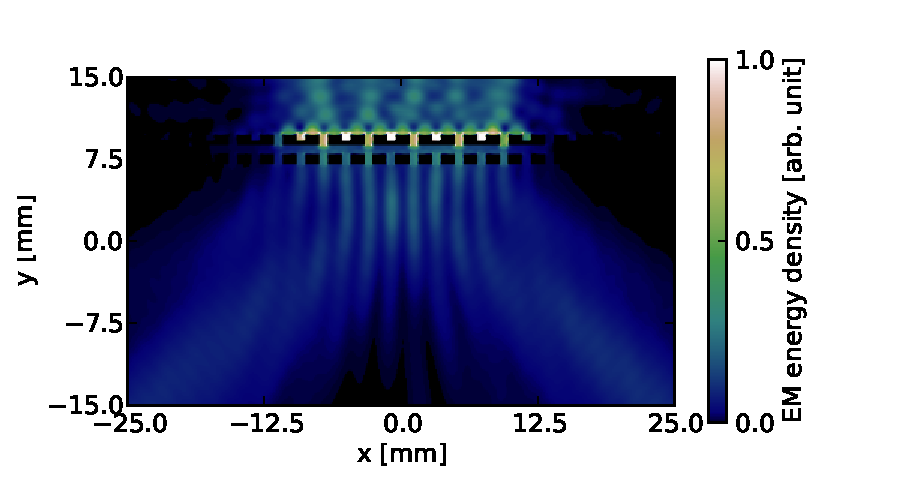
\includegraphics[width=3.5 in]{fig2a.eps}\\
 \vspace{.3 cm}
 (b)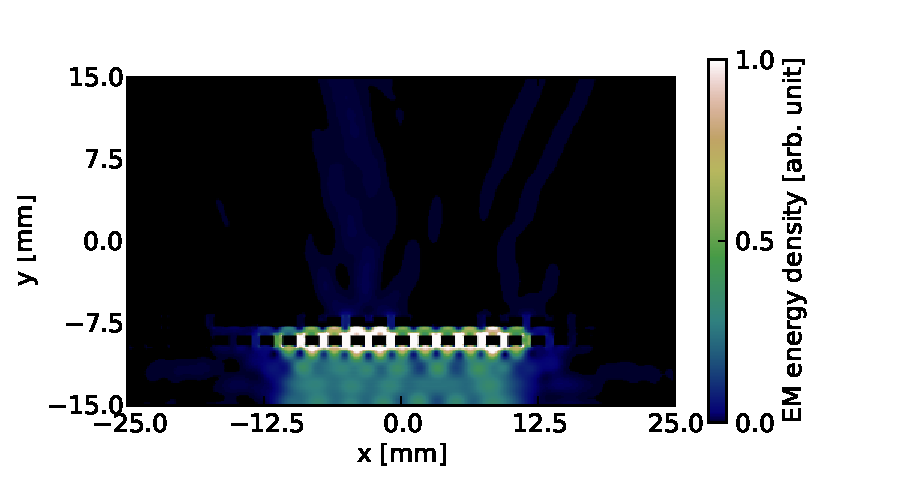
\includegraphics[width=3.5 in]{fig2b.eps}
\end{center}
\caption{Distributions of the energy density calculated with FDTD at the frequency of $0.1$~THz for the two opposite directions of incidence. (a) incidence from the top side, transmission in the $\pm1$ orders; (b) incidence from the bottom side, transmission is suppressed.\label{fig.fdtdfield}}
\end{figure}

\begin{figure}
 \begin{center}
 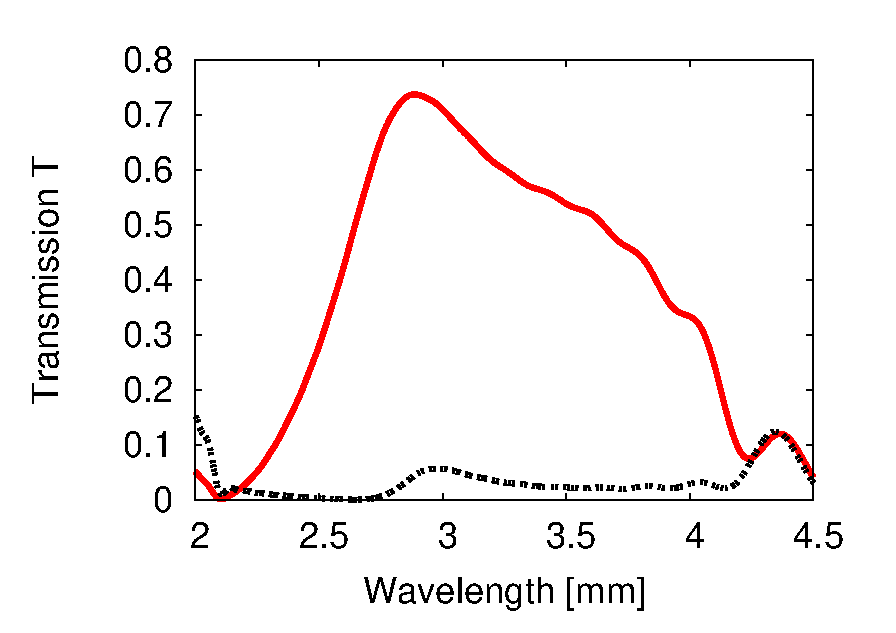
\includegraphics[width=3in]{fig3.eps}
\end{center}
\caption{Total transmission spectra $T(\lambda)$ of the double grating calculated using FDTD in the two opposite directions. Continuous line (red on-line) corresponds to the incidence from the top side, black dashed line denotes the incidence from the bottom side.\label{fig.spectra}}
\end{figure} 



We have optimized the double grating structure for a broadband unidirectional transmission with the central frequency of $0.1$ THz. The metallic element consists of a stack of $0.1$ mm thick slices made of stainless steel. In the FDTD simulations aimed at optimization of the structure, the metal is assumed to be a perfect conductor, a Gaussian pulse is used to determine the transmission spectrum, and periodic boundary conditions are imposed to terminate the computational mesh. Similar simulations with CW illumination, and with a finite size of the grating containing $10$ periods terminated with perfectly matched layer boundary conditions give consistent results, with the difference in transmission spectra smaller than $2\%$. An example of the field distribution obtained with a CW source is presented in Fig.~\ref{fig.fdtdfield}. Supplementary RCWA simulations gave only a qualitative confirmation of the device operation due to convergence problems resulting from the attempt to use a Fourier harmonic expansion 
for highly conducting materials with abrupt subwavelength boundaries. FDTD results showing a possibility to achieve 
broadband ($\lambda\sim 2$--$4$~mm) unidirectional transmission are presented in Fig.~\ref{fig.spectra}. The respective optimized geometric parameters are the following: $\Lambda_1=2\Lambda_2=4.2$~mm, $a_1=a_2=a_3=0.7$~mm, $h_1=h_2=2 h_0=1$~mm. 

%Secondly to check spatial field distribution we simulate finite length DMG illuminated by monochromatic source of wavelength $\lambda=3\text{mm}$. 

\begin{figure}
 \begin{center} 
 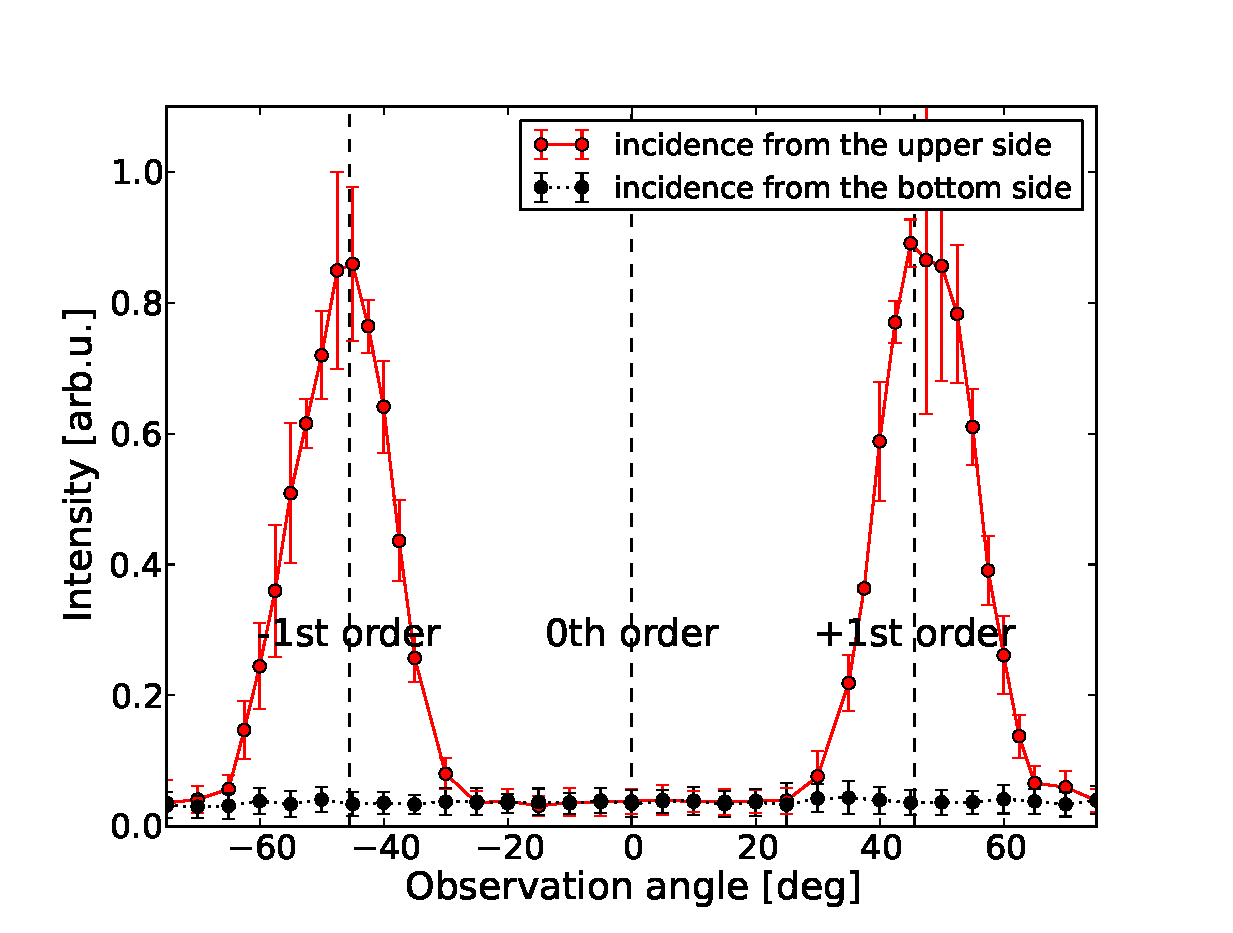
\includegraphics[width=3in]{fig4.eps}
\end{center}
\caption{Intensity of the angular transmission spectrum  of the double grating measured at the frequency of $0.1$~THz in both directions. \label{fig.experim}}
\end{figure} 

\begin{figure}
 \begin{center}
 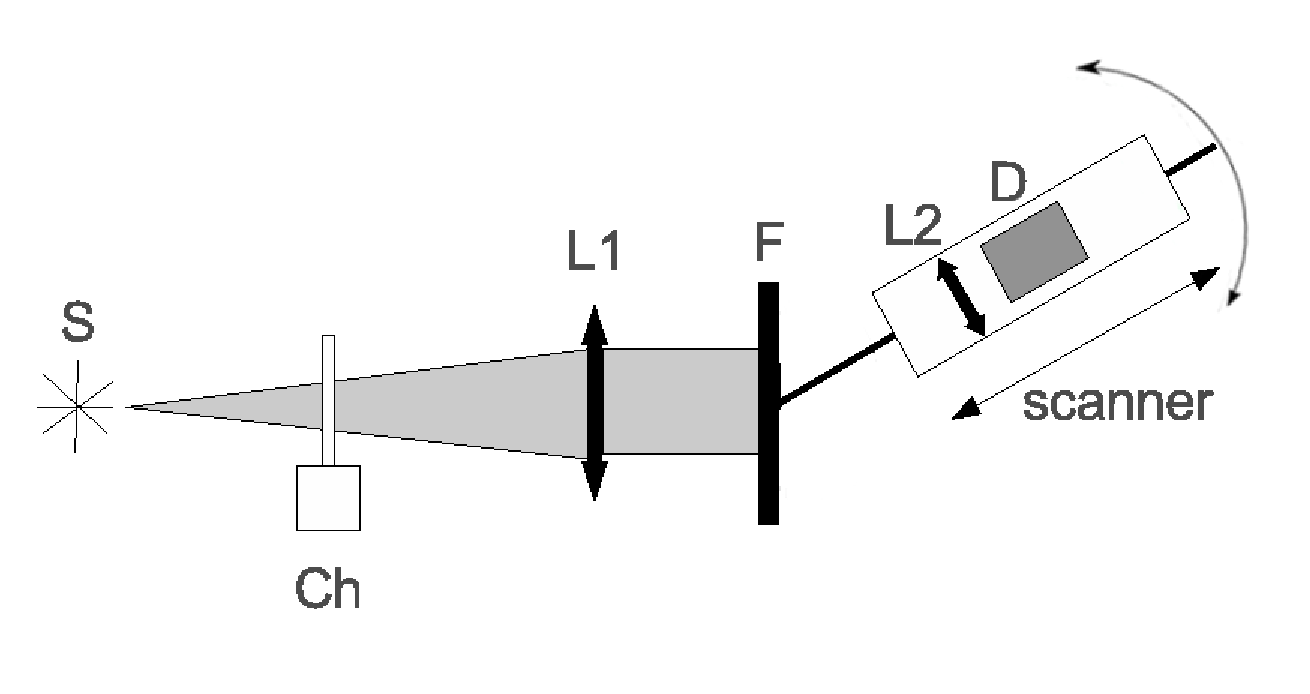
\includegraphics[width=3in]{fig5.eps}
\end{center}
\caption{Measurement set-up (S - Gunn diode, Ch - chopper, F - asymmetric filter, L1,L2 - PTFE lenses, D detector.)\label{fig.setup}}
\end{figure} 

We have measured the angular transmission spectrum of the dual grating in the frequency range of $0.095$--$0.110$~THz at room temperature, and the results for $0.1$~THz are shown in Fig.~\ref{fig.experim}. The experimental set-up is presented in Fig.~\ref{fig.setup}. The size of the grating is $42$~mm$\times 42$~mm,  the beam diameter is approximately equal to $2$~cm, a PTFE (Teflon \texttrademark) lenses are used to control the divergence of the beam. Measurements are consistent with FDTD simulations, transmission is observed only in the $\pm1$ diffraction orders and only in one direction, the suppressed  orders are at the level of the background noise (Signal to noise ratio SNR$\sim20$--$30$~dB). Reciprocity in the 0th order is evident from Fig.~\ref{fig.experim}. 
%Averaged total energy field distributions in stable state for both directions of wave propagation are shown in Fig.~\ref{fig.experim}.

In conclusion, we have optimized a double metallic grating for a broadband unidirectional transmission in the THz frequency range. Its operation is reciprocal, despite previous reports of zero order nonreciprocity.  The filter has an asymmetric transmission in one direction in the $\pm1$ diffraction orders, and blocks the $0$th order, a high extinction ratio is confirmed experimentally at $0.1$~THz.

This work is supported by the research projects of the Polish National Science Center
UMO-2011/01/M/ST3/05734, UMO-6081/B/TO2/2010/39 and UMO-2011/01/B/ST3/02281. CJZR gratefully acknowledges a financial support from the Generalitat Valenciana (project ACOMP/2012/003).

\bigskip



\begin{thebibliography}{10}
\newcommand{\enquote}[1]{``#1''}

\bibitem{1}
M. Scalora, J. P. Dowling, C. M. Bowden, and M. J. Bloemer, 
%``The photonic band edge optical diode,'' 
J. Appl. Phys. \textbf{76}, 2023 (1994).

\bibitem{1b}
Z. Wang, Y. D. Chong, J. D. Joannopoulos, and Marin Soljacic, 
%``Reflection-Free One-Way Edge Modes in a Gyromagnetic Photonic Crystal,''
Phys. Rev. Lett. \textbf{100}, 013905 (2008).

\bibitem{12}
A. S. Schwanecke, V. A. Fedotov, V. V. Khardikov, S. L. Prosvirnin, Y. Chen, and N. I. Zheludev,
%``Nanostructured Metal Film with Asymmetric Optical Transmission,''
Nano Lett. \textbf{8},  2940 (2008).

\bibitem{2}
M. J. Lockyear, A. P. Hibbins, K. R. White, and J. R. Sambles,
%``One-way diffraction grating,''
Phys. Rev. E \textbf{74}, 056611 (2006).

\bibitem{3}
A. Mandatori, M. Bertolotti, and C. Sibilia, 
%``Asymmetric transmission of some two-dimensional photonic crystals,''
J. Opt. Soc. Am. B \textbf{24}, 685(2007).

\bibitem{4}
A. E. Serebryannikov, 
%``One-way diffraction effects in photonic crystal gratings made of isotropic materials,'' 
Phys. Rev. B \textbf{80}, 155117 (2009).

\bibitem{5}
H. Kurt, D. Yilmaz, A. E. Akosman, and E. Ozbay, 
%``Asymmetric light propagation in chirped photonic crystal waveguides,'' 
Opt. Express \textbf{20}, 20635 (2012). 

\bibitem{6}
S. Cakmakyapan, A. E. Serebryannikov, H. Caglayan, and E. Ozbay, 
%``One-way transmission through the subwavelength slit in nonsymmetric metallic gratings,''
Opt. Lett. \textbf{35}, 2597 (2010). 

\bibitem{7}
S. Cakmakyapan, H. Caglayan, A. E. Serebryannikov, and E. Ozbay,
%``Experimental validation of strong directional selectivity in nonsymmetric metallic gratings with a subwavelength slit,''
Appl. Phys. Lett. \textbf{98}, 051103 (2011).

\bibitem{8}
E. Battal, T. A. Yogurt, and A. K. Okyay,
%``Ultrahigh Contrast One-Way Optical Transmission Through a Subwavelength Slit,''
Plasmonics DOI 10.1007/s11468-012-9419-4.

\bibitem{9}
P. Wr\a'{o}bel, J. Pniewski, T. J. Antosiewicz, and T. Szoplik,
%``Focusing radially polarized light by concentrically corrugated silver film without a hole,''
Phys. Rev. Lett. \textbf{102}, 183902 (2009).

\bibitem{10}
P. Wr\a'{o}bel, T. J. Antosiewicz, J. Pniewski, and T. Szoplik,
%``Single-layer metal nanolenses with tight foci in far-field,'' 
Appl. Phys. A \textbf{103}, 821 (2011).

\bibitem{11}
V. Kuzmiak, and A. A. Maradudin, 
%``Asymmetric transmission of surface plasmon polaritons,'' 
Phys. Rev. A \textbf{86}, 043805 (2012).

\bibitem{13}
Chen Cheng, Jing Chen, Qi-Yang Wu, Fang-Fang Ren, Ji Xu, Ya-Xian Fan, and Hui-Tian Wang,
%``Controllable electromagnetic transmission based on dual-metallic grating structures composed of subwavelength slits,''  
Appl. Phys. Lett. \textbf{91}, 111111 (2007).

\bibitem{14}
Chen Cheng, Jing Chen, Da-Jian Shi, Qi-Yang Wu, Fang-Fang Ren, Ji Xu, Ya-Xian Fan, Jianping Ding, and Hui-Tian Wang,
%``Physical mechanism of extraordinary electromagnetic transmission in dual-metallic grating structures,''
Phys. Rev. B \textbf{78}, 075406 (2008).


\bibitem{17}
Ji Xu, Chen Cheng, Ming Kang, Jing Chen, Zhu Zheng, Ya-Xian Fan, and Hui-Tian Wang, 
%``Unidirectional optical transmission in dual-metal gratings in the absence of anisotropic and nonlinear materials,''
Opt. Lett. \textbf{36}, 1905 (2011). 

\bibitem{15}
Z. Marcet, J. W. Paster, D. W. Carr, J. E. Bower, R. A. Cirelli, F. Klemens, W. M. Mansfield, J. F. Miner, C. S. Pai, and H. B. Chan, 
%``Controlling the phase delay of light transmitted through double-layer metallic subwavelength slit arrays,''
Opt. Lett. \textbf{33}, 1410 (2008). %http://www.opticsinfobase.org/ol/abstract.cfm?URI=ol-33-13-1410

\bibitem{16}
Wei-Min Ye, Xiao-Dong Yuan, Chu-Cai Guo, and Chun Zen, 
%``Unidirectional transmission in non-symmetric gratings made of isotropic material,'' 
Opt. Express \textbf{18}, 7590 (2010).  



\bibitem{18}
Z. H. Zhu, K. Liu, W. Xu, Z. Luo, C. C. Guo, B. Yang, T. Ma, X. D. Yuan, and W. M. Ye, 
%``One-way transmission of linearly polarized light in plasmonic subwavelength metallic grating cascaded with dielectric grating,''
Opt. Lett. \textbf{37}, 4008 (2012).


\bibitem{19}
A. F. Oskooi, D. Roundy, M. Ibanescu, P. Bermel, J. D. Joannopoulos, and S. G. Johnson, 
%``MEEP: A flexible free-software package for electromagnetic simulations by the FDTD method,''
Comput. Phys. Comm. \textbf{181}, 687 (2010).

\bibitem{20}
%M. G. Moharam, D. A. Pommet, E. B. Grann and T. K. Gaylord, 
%%``Stable implementation of the rigorous coupled-wave analysis for surface-relief gratings: enhanced transmittance matrix approach,''
%J. Opt. Soc. Am. A \textbf{12}, 1077-1086 (1995). 
Ph. Lalanne, and G. M. Morris,
%``Highly improved convergence of the coupled-wave method for TM polarization,''
J. Opt. Soc. Am. A \textbf{13}, 779 (1996). 

\end{thebibliography}


\newpage
\begin{thebibliography}{10}
\newcommand{\enquote}[1]{``#1''}

\bibitem{1}
M. Scalora, J. P. Dowling, C. M. Bowden, and M. J. Bloemer, 
``The photonic band edge optical diode,'' 
J. Appl. Phys. \textbf{76}, 2023 (1994).

\bibitem{1b}
Z. Wang, Y. D. Chong, J. D. Joannopoulos, and Marin Soljacic, 
``Reflection-Free One-Way Edge Modes in a Gyromagnetic Photonic Crystal,''
Phys. Rev. Lett. \textbf{100}, 013905 (2008).

\bibitem{12}
A. S. Schwanecke, V. A. Fedotov, V. V. Khardikov, S. L. Prosvirnin, Y. Chen, and N. I. Zheludev,
``Nanostructured Metal Film with Asymmetric Optical Transmission,''
Nano Lett. \textbf{8},  2940--2943 (2008).

\bibitem{2}
M. J. Lockyear, A. P. Hibbins, K. R. White, and J. R. Sambles,
``One-way diffraction grating,''
Phys. Rev. E \textbf{74}, 056611 (2006).

\bibitem{3}
A. Mandatori, M. Bertolotti, and C. Sibilia, 
``Asymmetric transmission of some two-dimensional photonic crystals,''
J. Opt. Soc. Am. B \textbf{24}, 685-690 (2007).

\bibitem{4}
A. E. Serebryannikov, 
``One-way diffraction effects in photonic crystal gratings made of isotropic materials,'' 
Phys. Rev. B \textbf{80}, 155117 (2009).

\bibitem{5}
H. Kurt, D. Yilmaz, A. E. Akosman, and E. Ozbay, 
``Asymmetric light propagation in chirped photonic crystal waveguides,'' 
Opt. Express \textbf{20}, 20635--20646 (2012). 

\bibitem{6}
S. Cakmakyapan, A. E. Serebryannikov, H. Caglayan, and E. Ozbay, 
``One-way transmission through the subwavelength slit in nonsymmetric metallic gratings,''
Opt. Lett. \textbf{35}, 2597--2599 (2010). 

\bibitem{7}
S. Cakmakyapan, H. Caglayan, A. E. Serebryannikov, and E. Ozbay,
``Experimental validation of strong directional selectivity in nonsymmetric metallic gratings with a subwavelength slit,''
Appl. Phys. Lett. \textbf{98}, 051103 (2011).

\bibitem{8}
E. Battal, T. A. Yogurt, and A. K. Okyay,
``Ultrahigh Contrast One-Way Optical Transmission Through a Subwavelength Slit,''
Plasmonics DOI 10.1007/s11468-012-9419-4.

\bibitem{9}
P. Wr\a'{o}bel, J. Pniewski, T. J. Antosiewicz, and T. Szoplik,
``Focusing radially polarized light by concentrically corrugated silver film without a hole,''
Phys. Rev. Lett. \textbf{102}, 183902 (2009).

\bibitem{10}
P. Wr\a'{o}bel, T. J. Antosiewicz, J. Pniewski, and T. Szoplik,
``Single-layer metal nanolenses with tight foci in far-field,'' 
Appl. Phys. A \textbf{103}, 821--825 (2011).

\bibitem{11}
V. Kuzmiak, and A. A. Maradudin, 
``Asymmetric transmission of surface plasmon polaritons,'' 
Phys. Rev. A \textbf{86}, 043805 (2012).

\bibitem{13}
Chen Cheng, Jing Chen, Qi-Yang Wu, Fang-Fang Ren, Ji Xu, Ya-Xian Fan, and Hui-Tian Wang,
``Controllable electromagnetic transmission based on dual-metallic grating structures composed of subwavelength slits,''  
Appl. Phys. Lett. \textbf{91}, 111111 (2007).

\bibitem{14}
Chen Cheng, Jing Chen, Da-Jian Shi, Qi-Yang Wu, Fang-Fang Ren, Ji Xu, Ya-Xian Fan, Jianping Ding, and Hui-Tian Wang,
``Physical mechanism of extraordinary electromagnetic transmission in dual-metallic grating structures,''
Phys. Rev. B \textbf{78}, 075406 (2008).


\bibitem{17}
Ji Xu, Chen Cheng, Ming Kang, Jing Chen, Zhu Zheng, Ya-Xian Fan, and Hui-Tian Wang, 
``Unidirectional optical transmission in dual-metal gratings in the absence of anisotropic and nonlinear materials,''
Opt. Lett. \textbf{36}, 1905--1907 (2011). 

\bibitem{15}
Z. Marcet, J. W. Paster, D. W. Carr, J. E. Bower, R. A. Cirelli, F. Klemens, W. M. Mansfield, J. F. Miner, C. S. Pai, and H. B. Chan, 
``Controlling the phase delay of light transmitted through double-layer metallic subwavelength slit arrays,''
Opt. Lett. \textbf{33}, 1410--1412 (2008). %http://www.opticsinfobase.org/ol/abstract.cfm?URI=ol-33-13-1410

\bibitem{16}
Wei-Min Ye, Xiao-Dong Yuan, Chu-Cai Guo, and Chun Zen, 
``Unidirectional transmission in non-symmetric gratings made of isotropic material,'' 
Opt. Express \textbf{18}, 7590--7595 (2010).  



\bibitem{18}
Z. H. Zhu, K. Liu, W. Xu, Z. Luo, C. C. Guo, B. Yang, T. Ma, X. D. Yuan, and W. M. Ye, 
``One-way transmission of linearly polarized light in plasmonic subwavelength metallic grating cascaded with dielectric grating,''
Opt. Lett. \textbf{37}, 4008--4010 (2012).


\bibitem{19}
A. F. Oskooi, D. Roundy, M. Ibanescu, P. Bermel, J. D. Joannopoulos, and S. G. Johnson, 
``MEEP: A flexible free-software package for electromagnetic simulations by the FDTD method,''
Comput. Phys. Comm. \textbf{181}, 687--702 (2010).

\bibitem{20}
%M. G. Moharam, D. A. Pommet, E. B. Grann and T. K. Gaylord, 
%%``Stable implementation of the rigorous coupled-wave analysis for surface-relief gratings: enhanced transmittance matrix approach,''
%J. Opt. Soc. Am. A \textbf{12}, 1077-1086 (1995). 
Ph. Lalanne, and G. M. Morris,
``Highly improved convergence of the coupled-wave method for TM polarization,''
J. Opt. Soc. Am. A \textbf{13}, 779--784  (1996). 

\end{thebibliography}
\end{document}
